\chapter{Findings}\label{chapter:findings}
This chapter collects the results of the individual models, the \ac{XAI} algorithms, and pattern recognition algorithms. The results are then analyzed and interpreted.

\section{Classification Models}
After doing all the preprocessing steps mentioned in chapter \ref{chapter:preprocessing}, the classification models have yielded the results visualized in figure \ref{fig:classification_performance}. The results indicate that ensemble methods, random forest and gradient boosting, seem to perform better than a classic random tree. The neural network classifier, however, performs best for all operations, with the exception of \textit{ycsb\_e\_init}, where gradient boosting performs better by a minimal difference of less than one percent. A surprising observation is the difference of performance between the initialization operations. This is attempted to be explained by the XAI techniques.
\begin{figure}[h]
      \centering
      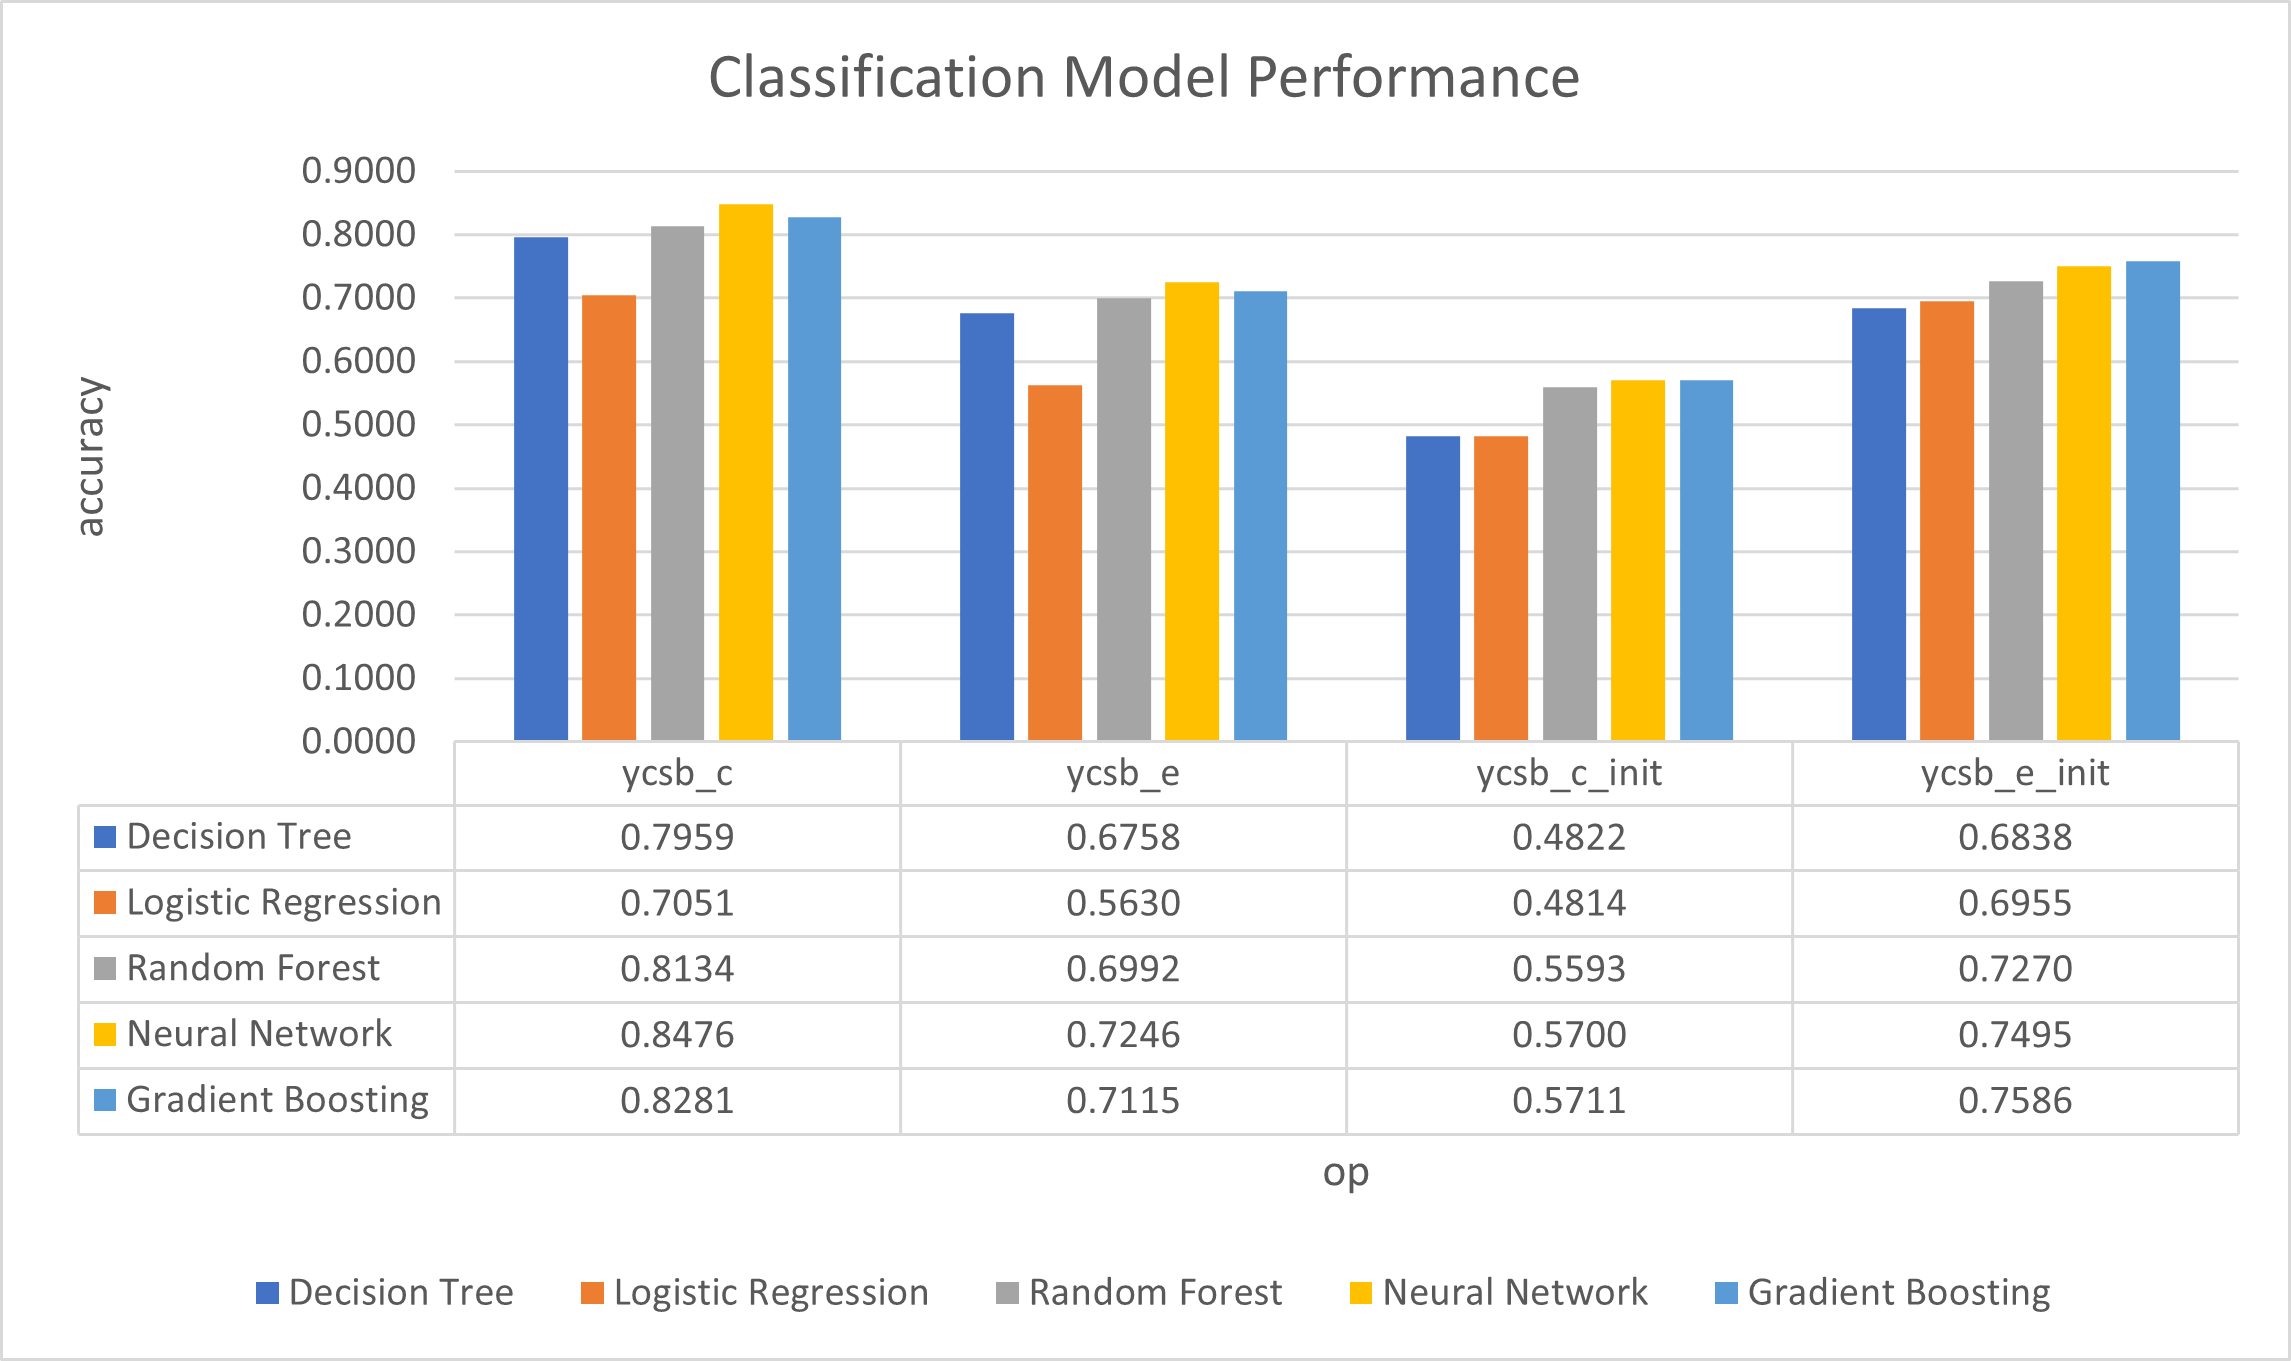
\includegraphics[width=0.85\textwidth]{images/classification_performance.png}
      \caption{Graph and data for performance of classification models}
      \label{fig:classification_performance}
  \end{figure}
\\\\
The generally best performing model in all cases, the neural network, has been further analyzed for each operation. This is done using \ac{XAI} techniques mentioned in chapter \ref{chapter:xai}. It should be noted that similar figures have been created for the gradient boosting models during experimentation, and therefore only the insights from the best performing models are shown and discussed. \\

\subsection{Permutation Feature Importance}
Figure \ref{fig:nnfeatimp} depicts four box-plots generated by applying the permutation feature importance algorithm on the neural networks created for the four operation types.
\begin{figure}[h]
      \centering
      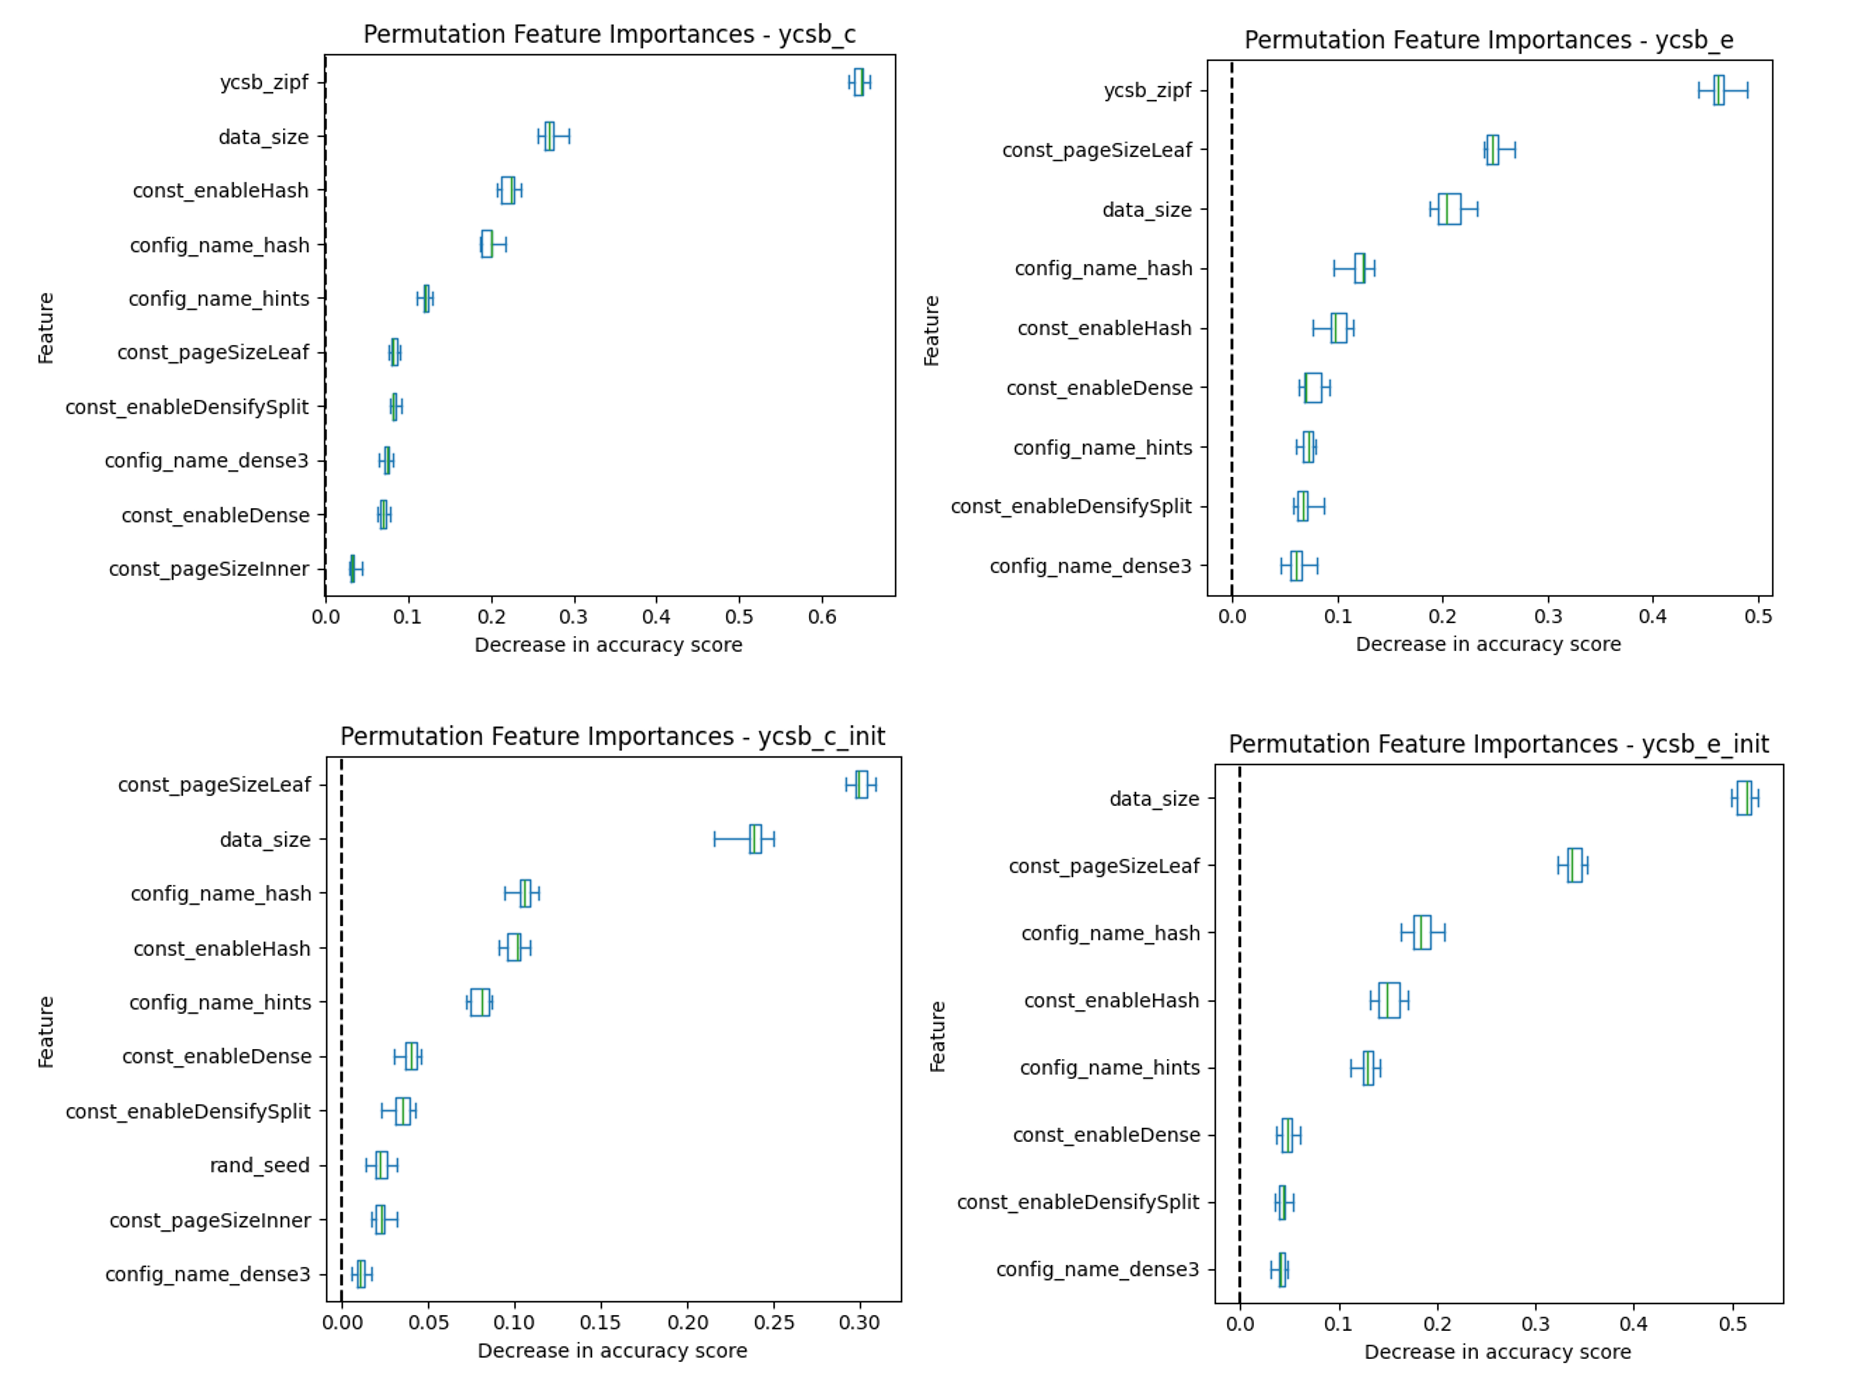
\includegraphics[width=0.9\textwidth]{images/nn_fi.png}
      \caption{Neural network permutation feature importances}
      \label{fig:nnfeatimp}
  \end{figure}
\\\\
The most notable result is that the feature \textit{ycsb\_zipf}, which describes how skewed the distribution of accessed keys is, is the most important feature for the benchmarking operations. For the initialization, the feature has no importance, which can be explained by the fact that the initialization operations do not consider the skewness during the run. 
\\\\
Furthermore, it can be seen that for operations that perform insertions (\textit{ycsb\_e}, \textit{ycsb\_e\_init}, \textit{ycsb\_c\_init}) the feature \textit{const\_pageSizeLeaf} has a higher importance. The \textit{data\_size} is important for all operations, which can be explained by the fact that the B+ tree grows with more data and therefore the operations require more time to read and insert.
\\\\
Since the features \textit{const\_enableHash} and \textit{config\_name\_hash} are highly correlated, it is understandable why the features are assigned similar importance. The slight differences could be explained by the random permutations that occur during the creation of the plot. 
\\\\
One should not assume that a higher importance of a configuration name implies a better performance. For example, the higher importance of \textit{config\_name\_hash} than \textit{config\_name\_dense3} only implies that when the models classify more based on the \textit{config\_name\_hash} than \textit{config\_name\_dense3}. To understand which configurations lead to which classification, one could use local \ac{XAI} techniques or use pattern recognition to identify these patterns. This, however, is beyond the objectives of this paper. 
\\\\
An unexplained phenomenon is the differences between the initialization operations. The feature \textit{data\_size} seems to be much more important for the operation \textit{ycsb\_e\_init}, compared to \textit{ycsb\_c\_init}. This could potentially explain the difference in the performance for the models. It could lie in the fact that for these two operations, the feature \textit{scale} is calculated differently, which impacts the target feature \textit{time} and consequently the models too. The feature \textit{scale} is set for the \textit{ycsb\_c\_init} to the number of keys, while for \textit{ycsb\_e\_init} $2.5\%$ is subtracted from that number. The subtraction is due to the fact that operation \textit{ycsb\_e} is expected to insert that amount of keys in its benchmark. However, validating this theory falls beyond the purview of this thesis.

\subsection{SHAP Summary Plot}
Figure \ref{fig:shap_sum} depicts four SHAP summary plots generated by applying the KernelSHAP algorithm and plotting the results of the neural networks created for the four operation types.
\begin{figure}[h]
      \centering
      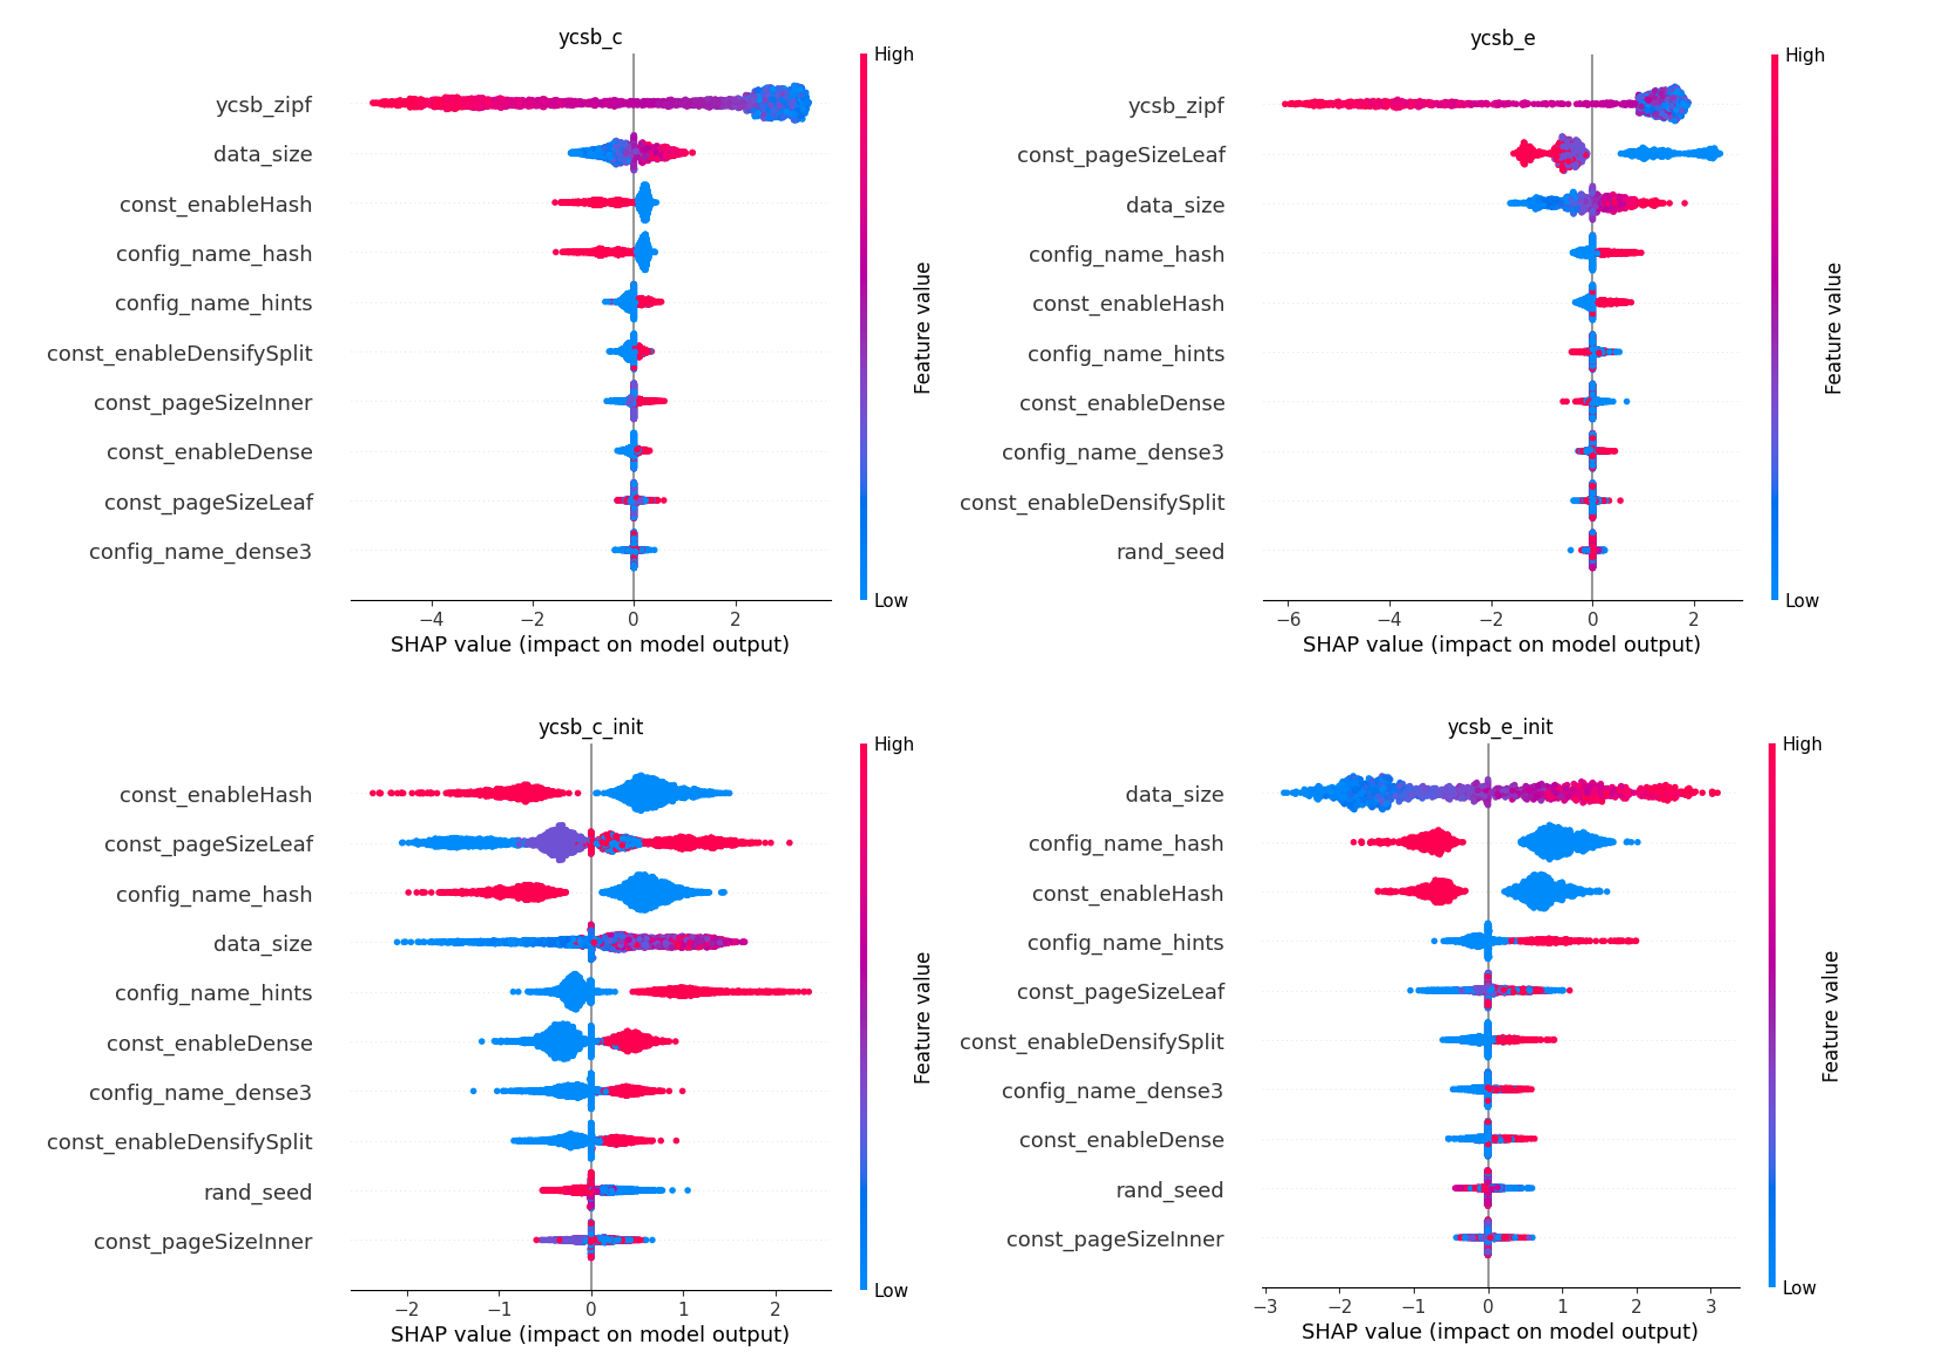
\includegraphics[width=0.9\textwidth]{images/shap_sum.png}
      \caption{Neural network SHAP summary plots per operation}
      \label{fig:shap_sum}
  \end{figure}
\\\\
Comparing the results between permutation feature importance plots and SHAP summary plots, the SHAP summary plots corroborate the conclusions drawn from the permutation feature importance plots. The SHAP summary plots, however, provide a few more insights. The colors in figure \ref{fig:shap_sum} indicate the plot relative feature value, with low values being blue and high values being red. These colors can then be compared with the Shapley values. For example, a cluster of blue dots for a feature on the positive side of the x-axis indicates that low values of the feature result in a higher target class, meaning a lower performance. 
\\\\
Based on this, it can be concluded that higher values of feature \textit{ycsb\_zipf} result in better performance for the operations \textit{ycsb\_c} and \textit{ycsb\_e}. The feature \textit{ycsb\_zipf} is generated randomly for each run between 0 and 1.5, with 0 meaning a normal distribution, 1 meaning a Zipfian distribution and above meaning even more skewed data. According to Claesen in \parencite{zipfdistr}, a Zipfian distribution indicates that fewer values are being accessed. Therefore, it can be interpreted that higher \textit{ycsb\_zipf} values indicate the cache can be better utilized, leading to better performance.
\\\\
For the feature \textit{data\_size} it is clearly visible at all operations that higher a smaller amount of data, leads to smaller trees and therefore a smaller class, meaning better performance. 
\\\\
Furthermore, for the initialization operations, one can notice that lower page sizes of leaf nodes result in better performance. This indicates that for the insertion operations benefit from lower leaf page sizes. Despite that, the \textit{ycsb\_e} figure could indicate a contradictory pattern, both patterns can be true. Considering that the \textit{ycsb\_e} consists of $95\%$ scan operations and only $5\%$ insertions, the scan operations outweigh the impact of the insertion operations. The scan operations, seem to benefit from higher leaf page sizes. This could be explained by the fact that higher leaf page sizes, lead to more consecutive values being stored in the same node and therefore during scan operations, fewer nodes need to be traversed. Insertion operations, on the other hand, might consider fewer values in a node more beneficial since it reduces the number of disk accesses required to write in a node. As a result, it can improve the performance of insertion operations, as disk I/O is often the bottleneck. This performance improvement seems to outweigh the drawback of having a higher depth and requiring more splitting operations. 

\section{Regression Models}
For regression models, the metrics have yielded the results depicted in figure \ref{fig:reg_mse} for metric MSE and figure \ref{fig:reg_r2} for metric $R^2$.
From these figures, one can conclude that the random forest model has yielded the best results in both metrics, with the exception of \textit{ycsb\_e\_init}, where the linear regression model performs better by a minimal margin.
\begin{figure}[H]
      \centering
      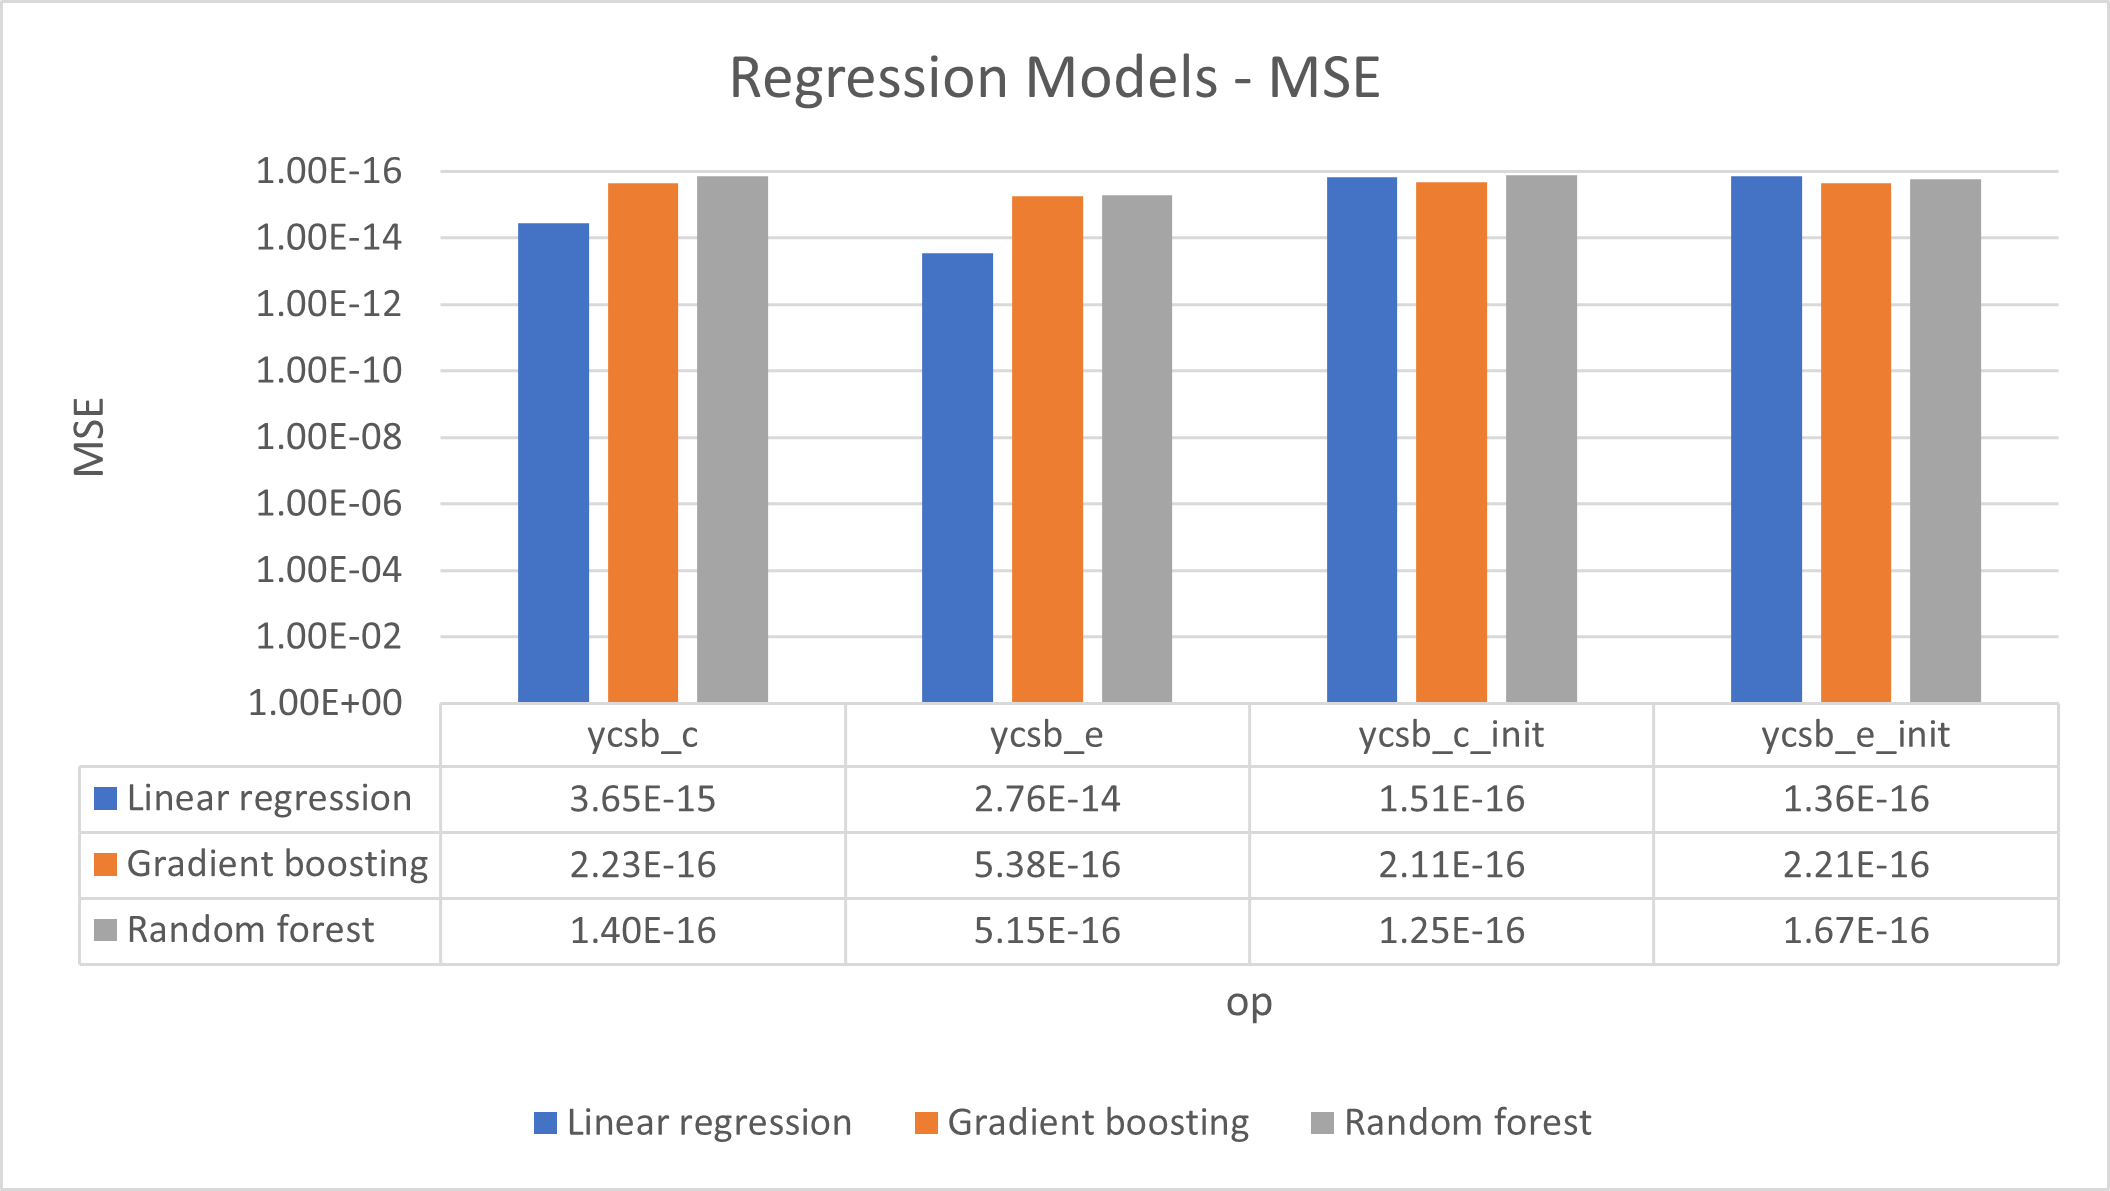
\includegraphics[width=0.8\textwidth]{images/reg_mse.png}
      \caption{Graph and data for MSE performance of regression models}
      \label{fig:reg_mse}
  \end{figure}
\begin{figure}[H]
      \centering
      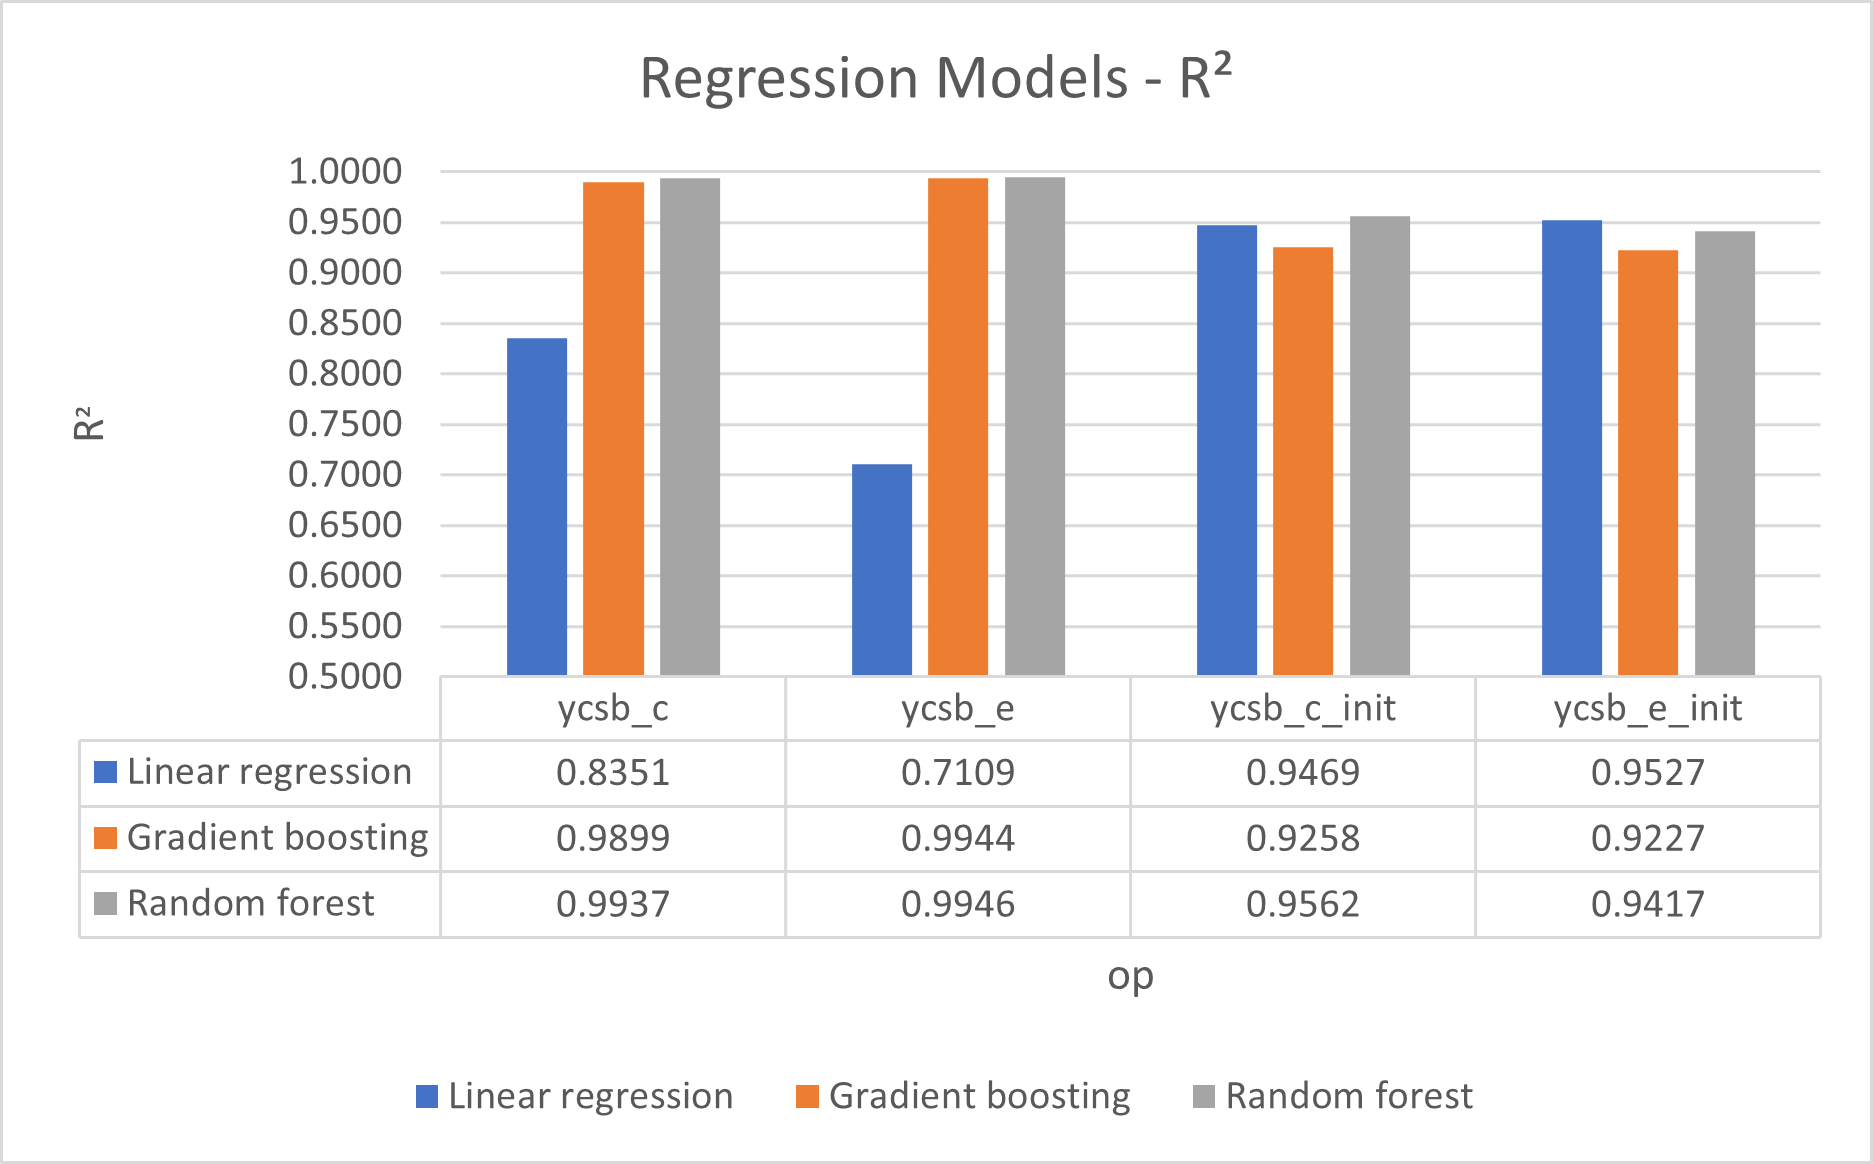
\includegraphics[width=0.8\textwidth]{images/reg_m2.png}
      \caption{Graph and data for $R^2$ performance of regression models}
      \label{fig:reg_r2}
  \end{figure}


\subsection{Permutation Feature Importance}
Producing insightful permutation feature importance plots has presented significant challenges, primarily stemming from the scale of the metrics and target feature. As a result, this particular step has been omitted from the scope of this thesis.\\

\subsection{SHAP Summary Plot}
Due to the scale of the target feature \textit{time}, the SHAP summary plots look differently, more clustered compared to the ones for classification. Nevertheless, similar outcomes can be deducted from the figure \ref{fig:shap_reg}. For example, the most important features remained the same, with only minor differences in order. Additionally, the same observations regarding features \textit{ycsb\_zipf}, \textit{const\_pageSizeLeaf} and \textit{data\_size} and their impact on the target feature can be made. However, due to the low interpretability caused by the scale of the target feature, the confidence for these statements is lower.


\begin{figure}[H]
      \centering
      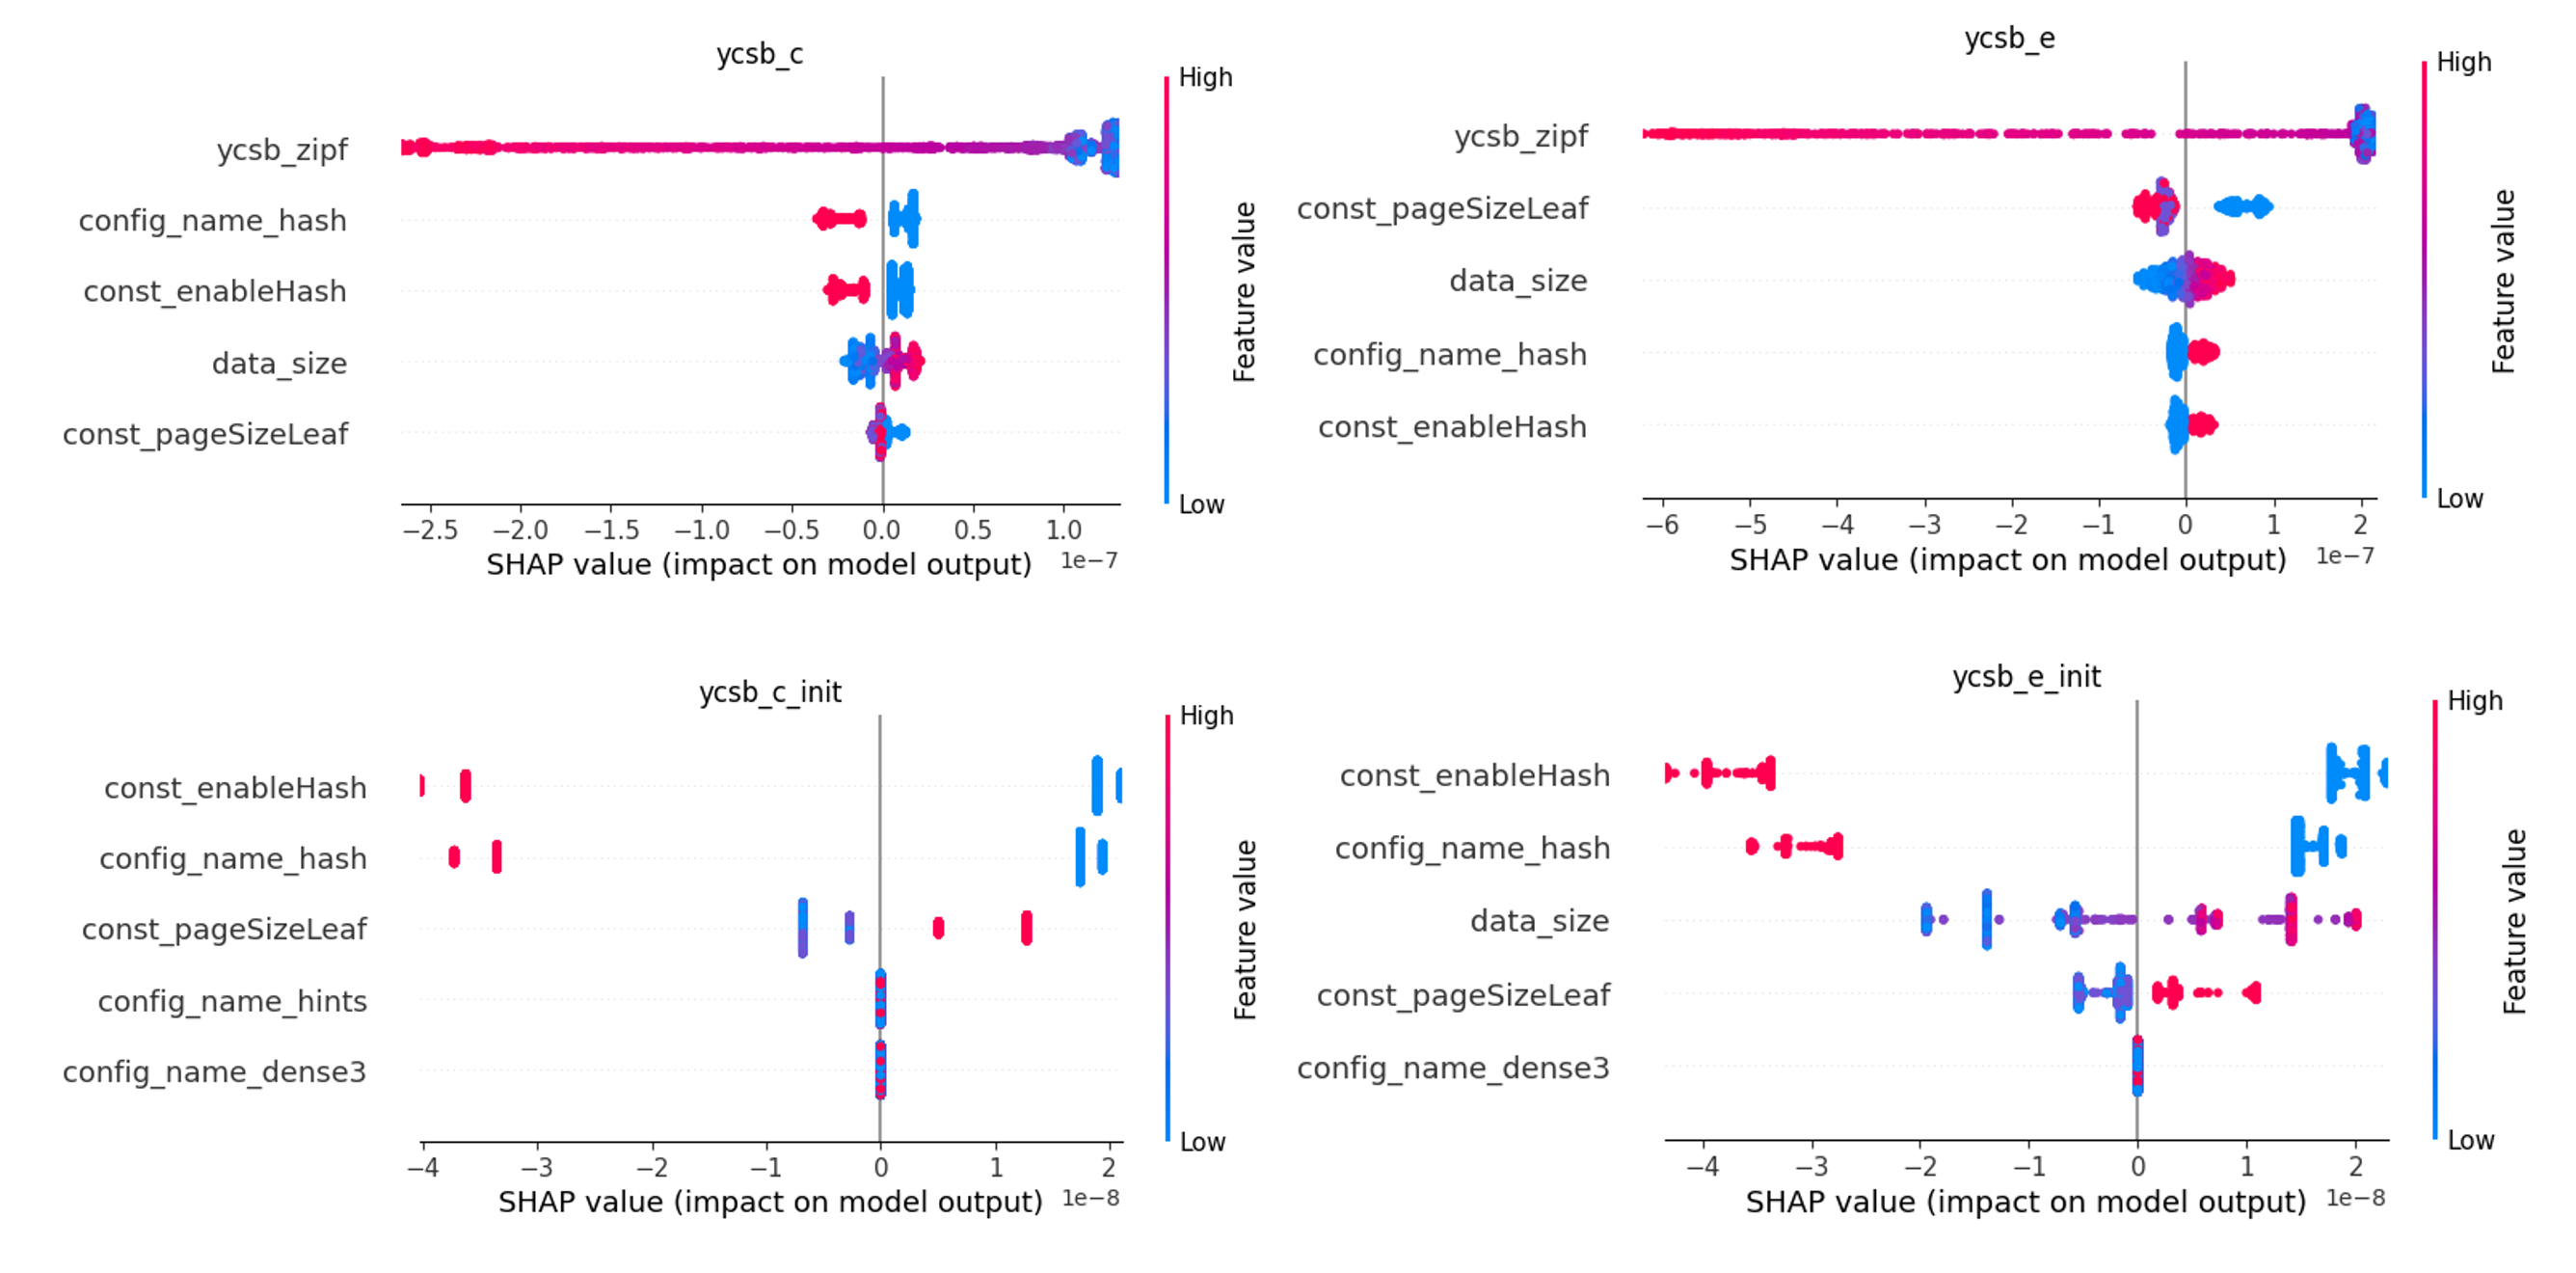
\includegraphics[width=0.95\textwidth]{images/shap_reg.png}
      \caption{Random forest SHAP summary plots per operation}
      \label{fig:shap_reg}
  \end{figure}




\section{Pattern recognition}
This section describes the results yielded by performing the Apriori algorithm and consequently the association rules mining algorithm. As described in chapter \ref{chapter:preprocessing} on preprocessing, the data used in this section is generated with a different data generation script than the one used for model training. The feature \textit{time}, is split into three buckets, as described, along with other necessary additional preprocessing steps, in section \ref{patternreg}. Bucket\_1 indicates the fastest times and therefore best performance.
\\\\
In the following results, the Apriori threshold has been set to $5\%$, and the association rules threshold for confidence to $40\%$. The result is then filtered to association rules, that are relevant to the performance. Additionally, to simplify the output, association rules that are redundant, by being majorly explained by a smaller antecedent, have been removed from the output. Furthermore, the consequent support is not displayed, since the buckets are split equally, meaning each has a support of close to $33\%$. Metrics not introduced in this thesis are also filtered out. 

\subsection{Association rules}

\textbf{ycsb\_c}:
As figure \ref{fig:pr_c} outlines, the major factor found for the purely read operation benchmark is feature \textit{data\_size}. Lower values for  \textit{data\_size} indicate better performance. Another notable result is that the biggest leaf page size for the benchmarking, 8192, tends to perform worst for this operation. 
\begin{figure}[h]
      \centering
      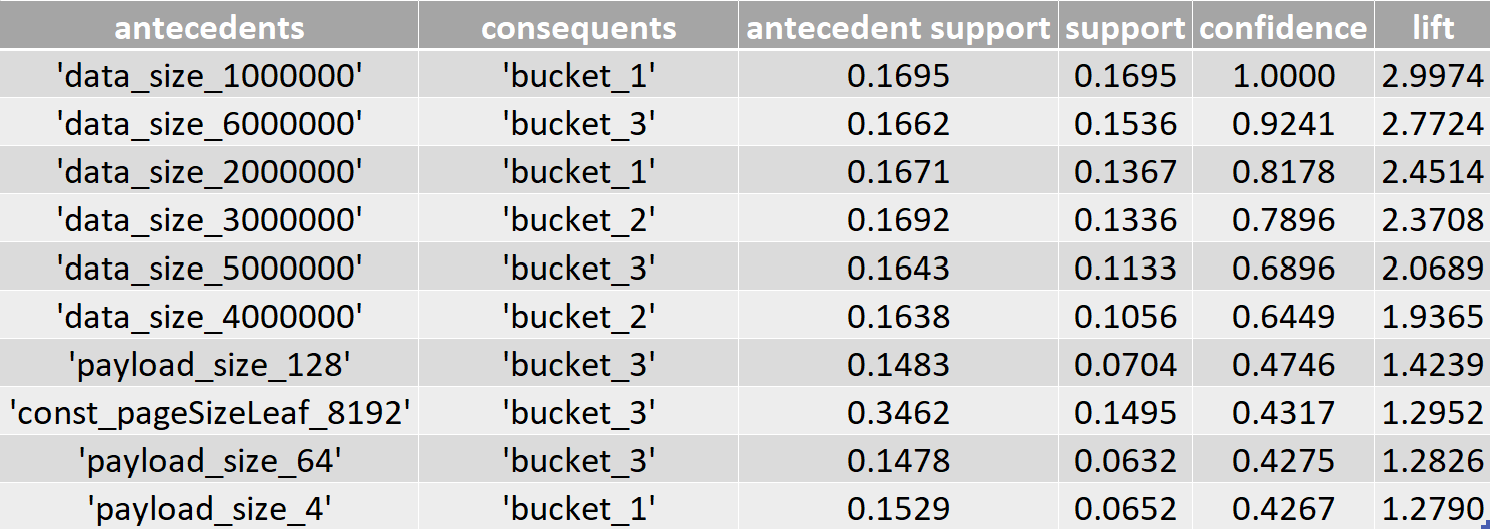
\includegraphics[width=0.6\textwidth]{images/pr_c.png}
      \caption{Association rules for \textit{ycsb\_c}}
      \label{fig:pr_c}
\end{figure}
\\\\
\textbf{ycsb\_e}:
For the operation \textit{ycsb\_e}, figure \ref{fig:pr_e} displays that the size of the payload is a decisive factor. For example, executions with payload size of 256, which occur about 10\% of the time in the dataset, end in the slowest bucket every time. Additionally, with the \textit{pageSizeLeaf} set to 2048, the executions mostly end up in the slowest two buckets, which considering that it is the lowest value in the dataset further underlines the findings from the previous section.
\begin{figure}[h]
      \centering
      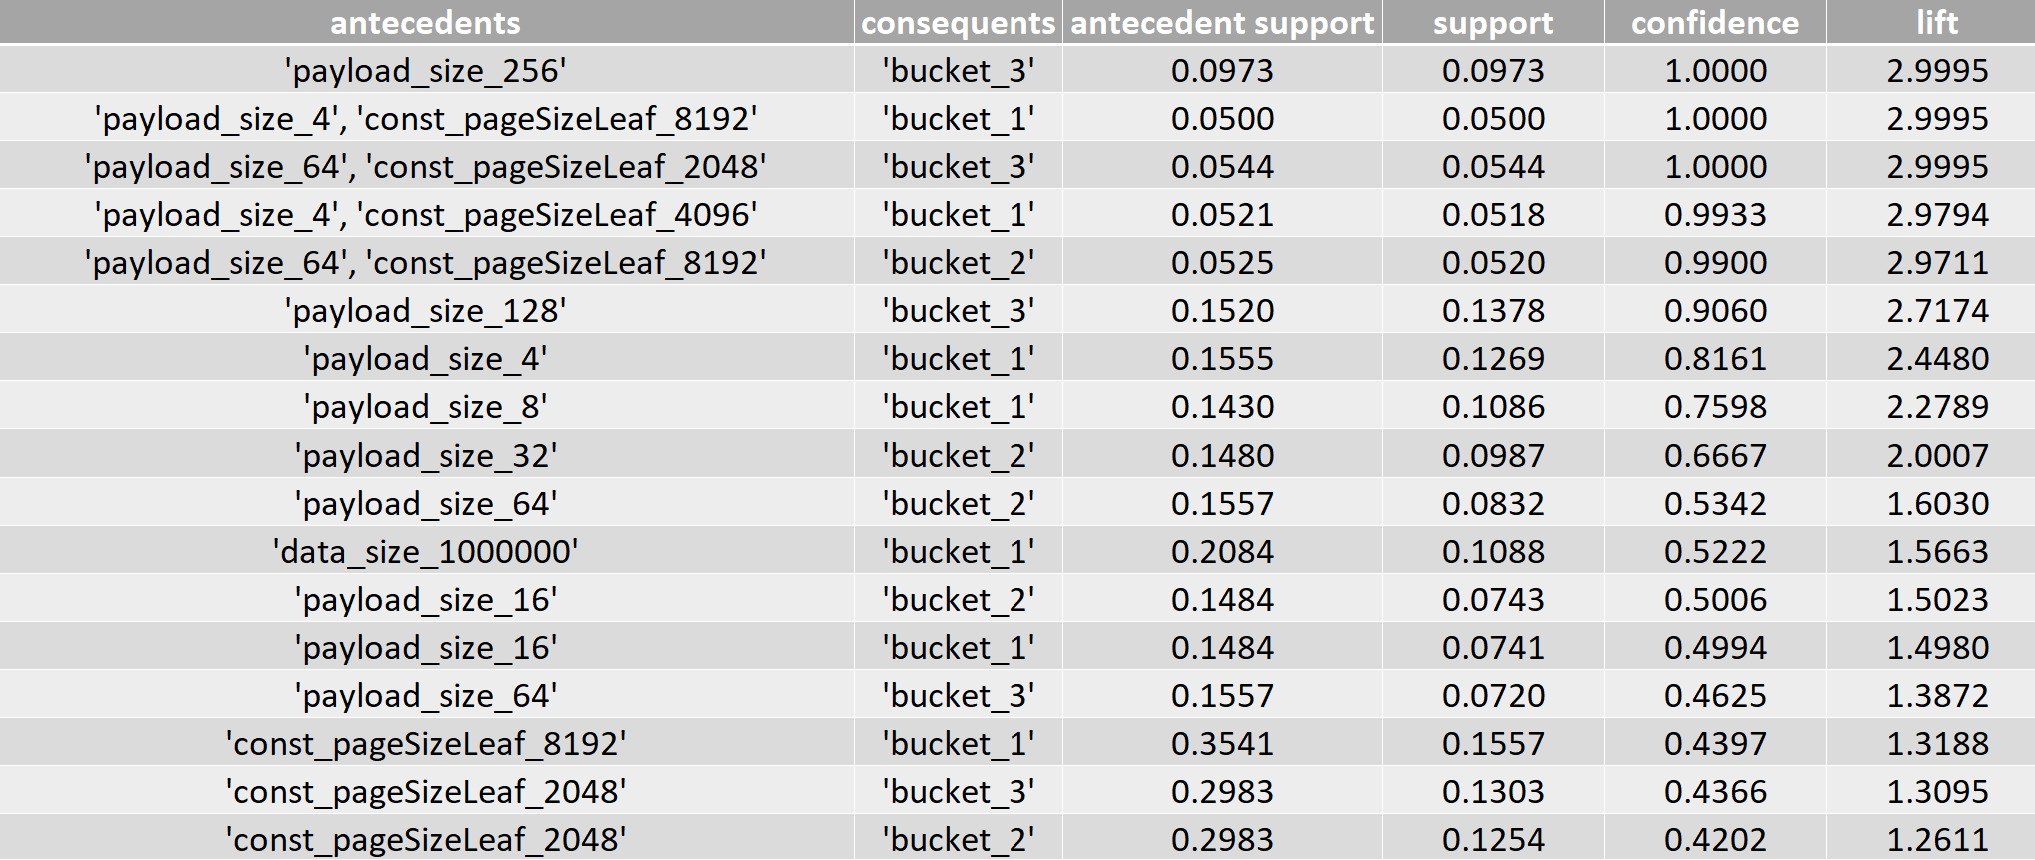
\includegraphics[width=0.6\textwidth]{images/pr_e.png}
      \caption{Association rules for \textit{ycsb\_e}}
      \label{fig:pr_e}
\end{figure}
\\\\
\textbf{ycsb\_c\_init}:
By looking at the figure \ref{fig:pr_c_init} one can observe a similar pattern, where the size of the payload and data can give a big indication, as to which of the three performance buckets the record belongs to. The pattern being that a high payload size indicates a slower performance. 
\begin{figure}[h]
      \centering
      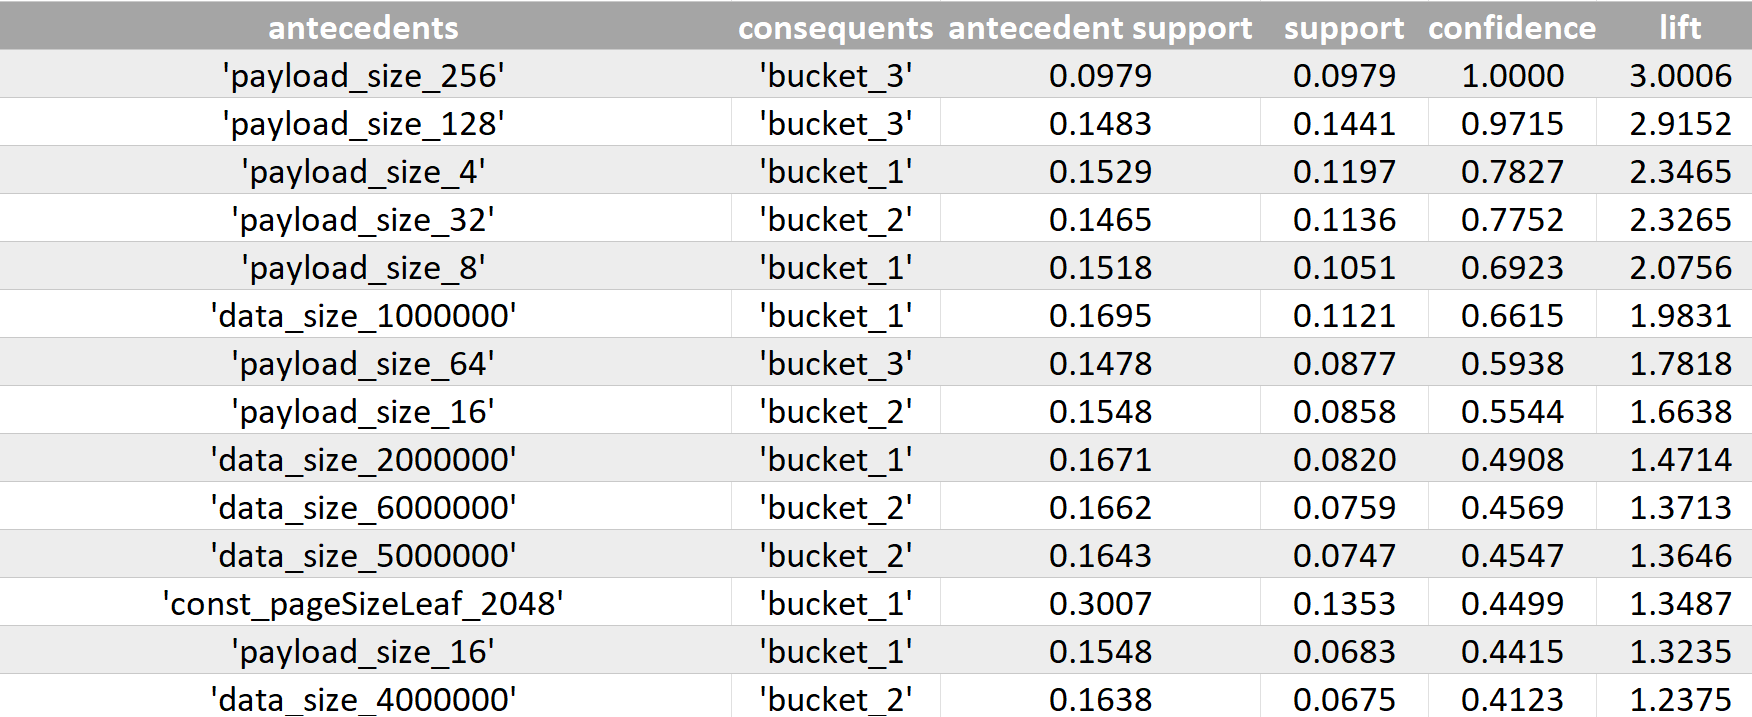
\includegraphics[width=0.6\textwidth]{images/pr_c_init.png}
      \caption{Association rules for \textit{ycsb\_c\_init}}
      \label{fig:pr_c_init}
\end{figure}
\\\\
\textbf{ycsb\_e\_init}:
The same observation as for operation \textit{ycsb\_c\_init} can be made for \textit{ycsb\_e\_init}. This is understandable, considering that these operations are very similar. The differences in values can be explained by the different scaling of feature \textit{time}. 
\begin{figure}[h]
      \centering
      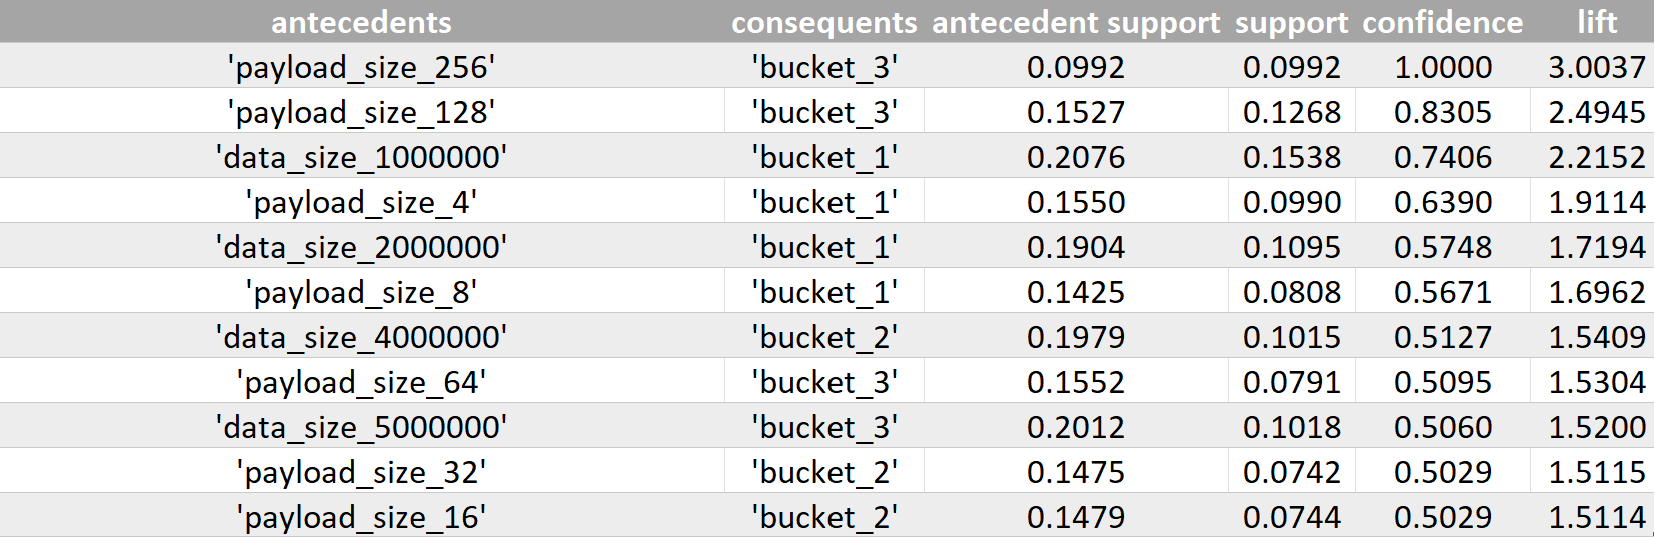
\includegraphics[width=0.6\textwidth]{images/pr_e_init.png}
      \caption{Association rules for \textit{ycsb\_e\_init}}
      \label{fig:pr_e_init}
\end{figure}


\subsection{Optimal page size of leaf nodes}
The methodology to generate heatmaps, based on regression models trained by the more discrete dataset, proved to be difficult. The output of the regression models, Random Forest and Gradient Boosting, as previous findings from the association rules indicate, greatly depends on the features \textit{payload\_size} and \textit{data\_size}. As a result, the various page sizes of leaf nodes received the same output based on features \textit{payload\_size} and \textit{data\_size}. Therefore, this methodology was not able to identify the optimal page size of leaf nodes. 
\\\\
Nevertheless, the heatmaps based on empirical means are generated and visualized in figure \ref{fig:heatmaps}.
\begin{figure}[h]
      \centering
      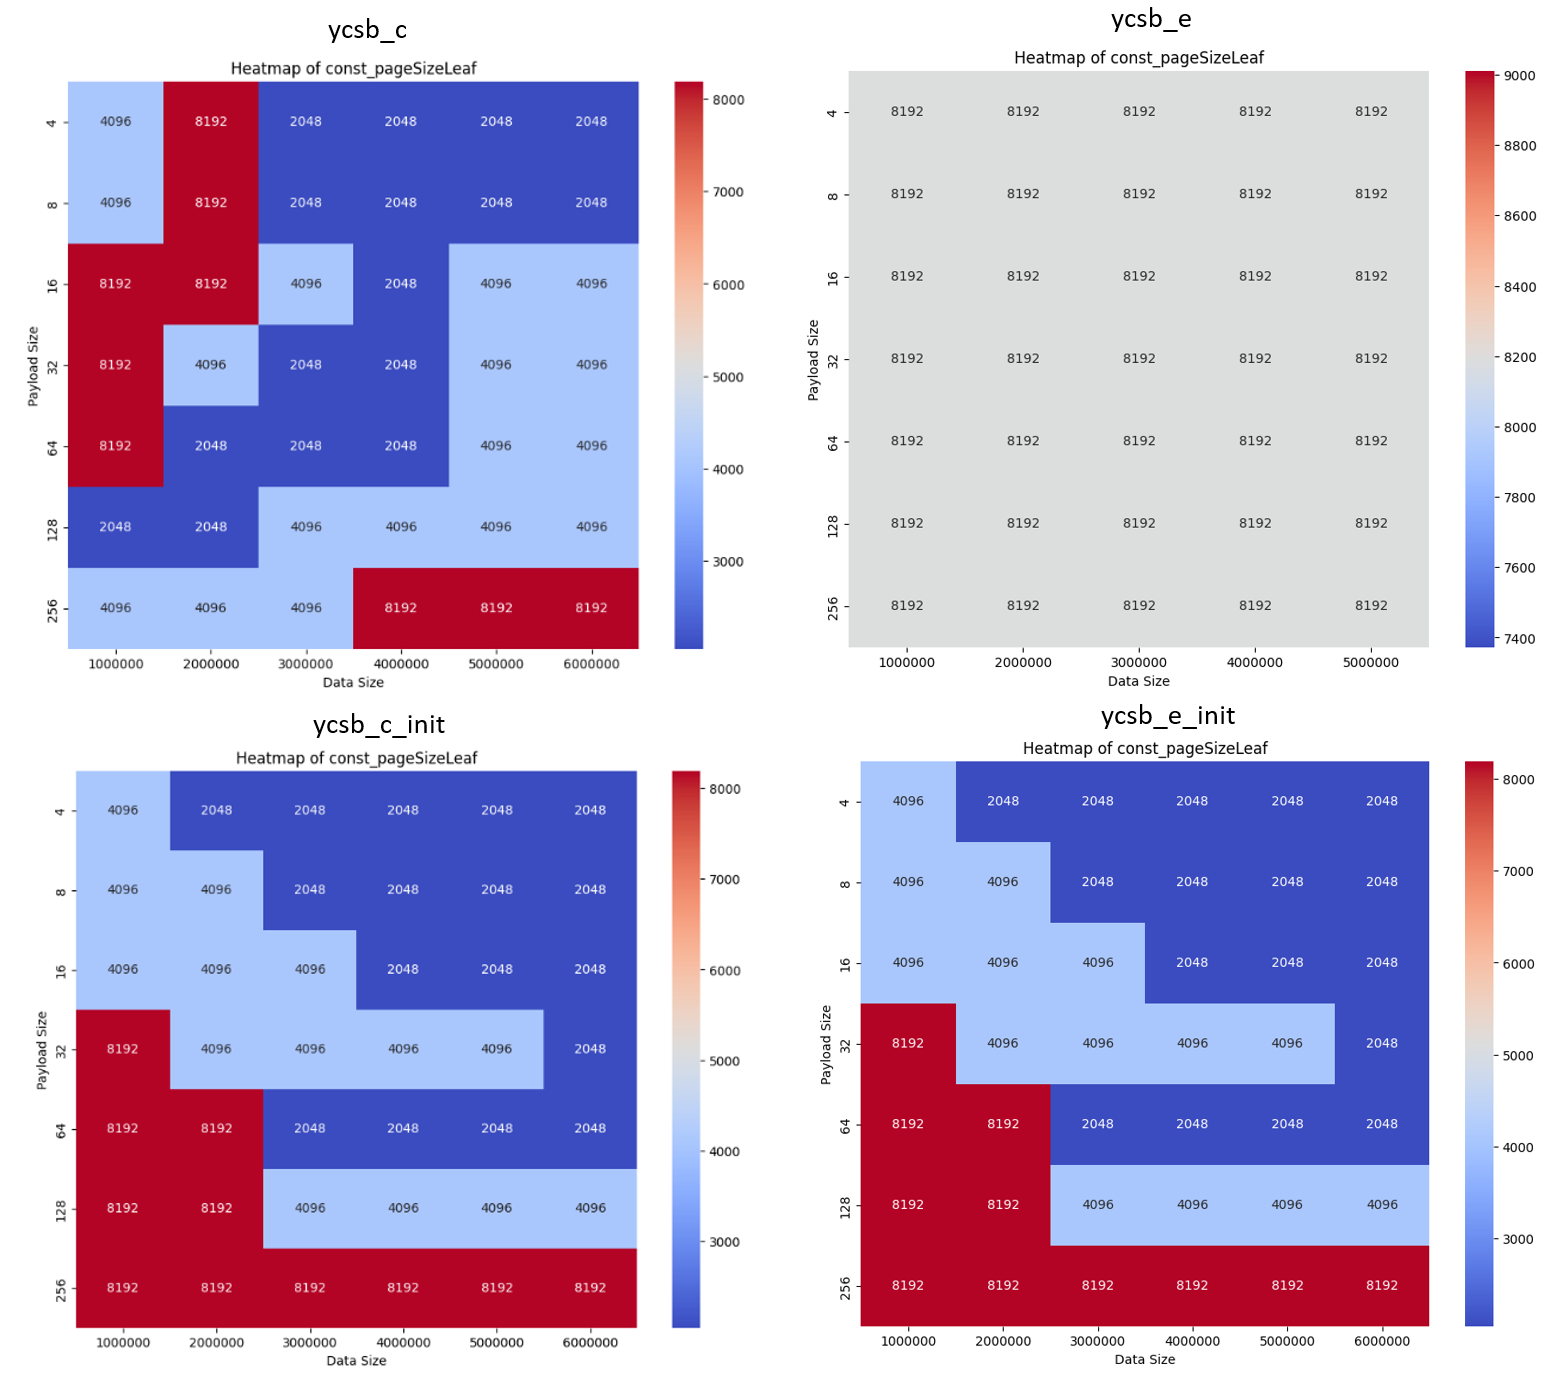
\includegraphics[width=0.95\textwidth]{images/heatmaps.png}
      \caption{Heatmaps per operation based on empirical mean}
      \label{fig:heatmaps}
\end{figure}
\\\\
The findings of operation \textit{ycsb\_e} indicate the high importance of big page sizes for scan operations. The page size 8192 is the highest in the data set, meaning that potentially a higher page size might be optimal. Operations {ycsb\_c\_init} and {ycsb\_e\_init} generated the same behavior, which is expected due to their similar nature. The pattern seems to indicate that during the insertion operations, higher sizes of the payload prefer higher page sizes, however, the bigger the size of the dataset, lower page sizes are preferred. These findings should be interpreted with caution, as the optimal page sizes generally result in only an $1-3\%$ improvement compared to the next best page size. Given that the values of the feature \textit{time} are in the order of magnitude of hundreds of nanoseconds  ($10^{-7}$ seconds), an $1-3\%$ improvement may not be considered substantial. Consequently, the heatmap for operation \textit{ycsb\_c} is not further analyzed. 